% \documentclass[aspectratio=169,notes]{beamer}
\documentclass[aspectratio=169]{beamer}
\usetheme[faculty=phil]{fibeamer}
\usepackage{polyglossia}
\setmainlanguage{english} %% main locale instead of `english`, you
%% can typeset the presentation in either Czech or Slovak,
%% respectively.
\setotherlanguages{russian} %% The additional keys allow
%%
%%   \begin{otherlanguage}{czech}   ... \end{otherlanguage}
%%   \begin{otherlanguage}{slovak}  ... \end{otherlanguage}
%%
%% These macros specify information about the presentation
\title[Theoretical Mechanics]{Theoretical Mechanics, Lab 12: DYN NEWTON EULER} %% that will be typeset on the
\subtitle{Approaches to dynamic modeling \\
Model-oriented design \\
Newton-Euler method } %% title page.
\author{Oleg Bulichev}
%% These additional packages are used within the document:
\usepackage{ragged2e}  % `\justifying` text
\usepackage{booktabs}  % Tables
\usepackage{tabularx}
\usepackage{tikz}      % Diagrams
\usetikzlibrary{calc, shapes, backgrounds}
\usepackage{amsmath, amssymb}
\usepackage{url}       % `\url`s
\usepackage{listings}  % Code listings
% \usepackage{subfigure}
\usepackage{floatrow}
\usepackage{subcaption}
\usepackage{mathtools}
\usepackage{todonotes}
\usepackage{fontspec}
\usepackage{multicol}
\usepackage{pdfpages}
\usepackage{wrapfig}
\usepackage{animate}
\usepackage{booktabs}
\usepackage{multirow}
% \usepackage{graphicx}
\usepackage{colortbl}
\usepackage{catchfilebetweentags}
\usepackage{makecell}
\graphicspath{{resources/}}
\frenchspacing

\setbeamertemplate{caption}[numbered]
\usetikzlibrary{graphs}

% \usepackage[backend=biber,style=ieee,autocite=footnote]{biblatex}
% \addbibresource{biblio.bib}
% \DefineBibliographyStrings{english}{%
%   bibliography = {References},}

\newcommand{\oleg}[2][] {\todo[color=red, #1] {OLEG:\\ #2}}
\newcommand{\fbckg}[1]{\usebackgroundtemplate{\includegraphics[width=\paperwidth]{#1}}}%frame background

\usepackage[framemethod=TikZ]{mdframed}
\newcommand{\dbox}[1]{
\begin{mdframed}[roundcorner=3pt, backgroundcolor=yellow, linewidth=0]
\vspace{1mm}
{#1}
\vspace{1mm}
\end{mdframed}
}

\begin{document}
\setlength{\abovedisplayskip}{0pt}
\setlength{\belowdisplayskip}{0pt}
\setlength{\abovedisplayshortskip}{0pt}
\setlength{\belowdisplayshortskip}{0pt}

\fbckg{fibeamer/figs/title_page.png}
\frame[c]{\setcounter{framenumber}{0}
    \usebeamerfont{title}%
    \usebeamercolor[fg]{title}%
    \begin{minipage}[b][6.5\baselineskip][b]{\textwidth}%
        \textcolor{black}{\raggedright\inserttitle}
    \end{minipage}
    % \vskip-1.5\baselineskip

    \usebeamerfont{subtitle}%
    \usebeamercolor[fg]{framesubtitle}%
    \begin{minipage}[b][3\baselineskip][b]{\textwidth}
        \raggedright%
        \insertsubtitle%
    \end{minipage}
    \vskip.25\baselineskip
}
%   \frame[c]{\maketitle}

\fbckg{fibeamer/figs/common.png}


\section*{Approaches to dynamic modeling }

\begin{frame}[t]{Three global approaches to dynamic modeling}
\framesubtitle{}
\scriptsize
\vspace{-0.8cm}
    \begin{columns}[T,onlytextwidth]
        \begin{column}{0.33\textwidth}
            \begin{center}
                \textbf{Modeling frameworks}
            \end{center}
            \vspace{-0.3cm}
            \textbf{Ex, Coding (1):} Pinocchio, RBDL

            \textbf{Ex, Model-oriented design (2):} MATLAB Simulink, SimInTech, Open Modelica
            \begin{itemize}
                \item[+] You understand your system fully and can control any part of it (1,2)
                \item[+] Easy to apply the solution to real system (1, 2)
                \item[+] Often open source frameworks (1)
                \item[+] For part of the tasks, no coding (2)
                \item[+] Fast solution for big systems (1)
                \item[-] Complicated to read and debug (1) (2 for big systems)
                \item[-] Big time consumptions (1)
            \end{itemize}
            \alert{Good for control applications (1,2)}
        \end{column}
        \begin{column}{0.33\textwidth}
            \begin{center}
                \textbf{Simulators}
            \end{center}
            \vspace{-0.3cm}
            \ \textbf{Ex:} Gazebo Sim, Mujoco, CoppeliaSim
            \begin{itemize}
                \item[+] No need to code dynamics, only description for a system
                \item[+] Made for simulating the system as whole (with sensors and so on) 
                \item[-] Need special software (most --- open source)
                \item[-] Not so easy to transfer the solution to a real system 
                \item[-] Physics models are rather simple. 
                \item[-] Often can't work with closed-loop systems
            \end{itemize}
            \alert{Well suit for simulate the whole system}
        \end{column}
        \begin{column}{0.33\textwidth}
            \begin{center}
                \textbf{Computer Aided Engineering (CAE)}
            \end{center}
            \vspace{-0.3cm}
            \textbf{Ex, CAE:} Siemens NX, ANSYS, Solid Works
            \begin{itemize}
                \item[+] The most intuitive systems (mostly interface based manipulation)
                \item[+] For most of the tasks, no coding
                \item[+] Physics models are quite complicated
                \item[-] Have to make a CAD model, even if the system is simple.
                \item[-] Need special software (most --- proprietary)
                \item[-] Very slow computations
            \end{itemize}
            \alert{Best for analyzing part of system}
        \end{column}
    \end{columns}
\end{frame}

\begin{frame}[t]{MaM HW CAE DYN1}
    \framesubtitle{}
    \vspace{-0.6cm}
        \begin{columns}[T,onlytextwidth]
            \begin{column}{0.59\textwidth}
                \scriptsize
        \textbf{Zip archive, which contains all needed data}: \textit{HWs/HW\_CAE\_DYN1/task\_data}
        
        1st joint is controllable, others --- not.
        \vspace{-0.1cm}
        \begin{enumerate}
            \item \textbf{Find angle limits} (where the mechanism stuck) for controllable joint:
            \vspace{-0.45cm}
    
            \begin{itemize}
                \scriptsize
                \item By code (solving kinematics problem for each angle)
                \item Using NX (either Modeling, or Animation Designer);
            \end{itemize}
            \vspace{-0.2cm}
    
            \item Compare results, present them as a pie chart in report.
            \item \textbf{Make the scene in Motion Analysis}. All links are made from <<Bronze>>. You need to add joints, contacts, direct earth gravity correctly.
            \item Choose the biggest angle gap between joint limits and put your link in the beginning of it.
            \item Apply constant angular acceleration for 1st joint --- 0.2 $rad / s^2$
            \item \textbf{Find a torque for 1st joint} for such angle gap:
            \vspace{-0.1cm}
    
            \begin{itemize}
                \scriptsize
                \item By code (solving Inverse dynamics problem)
                \item Using NX (any solver);
            \end{itemize}
            \vspace{-0.2cm}
    
            \item Compare results
        \end{enumerate}
            \end{column}
            \begin{column}{0.39\textwidth}
                \vspace{1cm}
                \begin{figure}[H]
                    \centering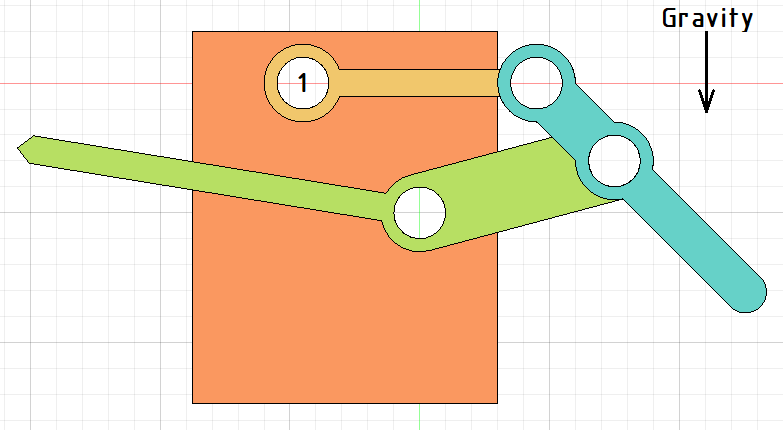
\includegraphics[height=6cm,width=1\textwidth,keepaspectratio]{task_descr.png}
                    % \caption{caption_name}
                    \label{fig:task_descr.png}
                \end{figure}
            \end{column}
        \end{columns}
    \end{frame}

\begin{frame}[t]{Solution (1)}
\framesubtitle{}
    \vspace{-0.6cm}
    \begin{figure}[H]
        \begin{subfigure}[t]{0.32\textwidth}
            \centering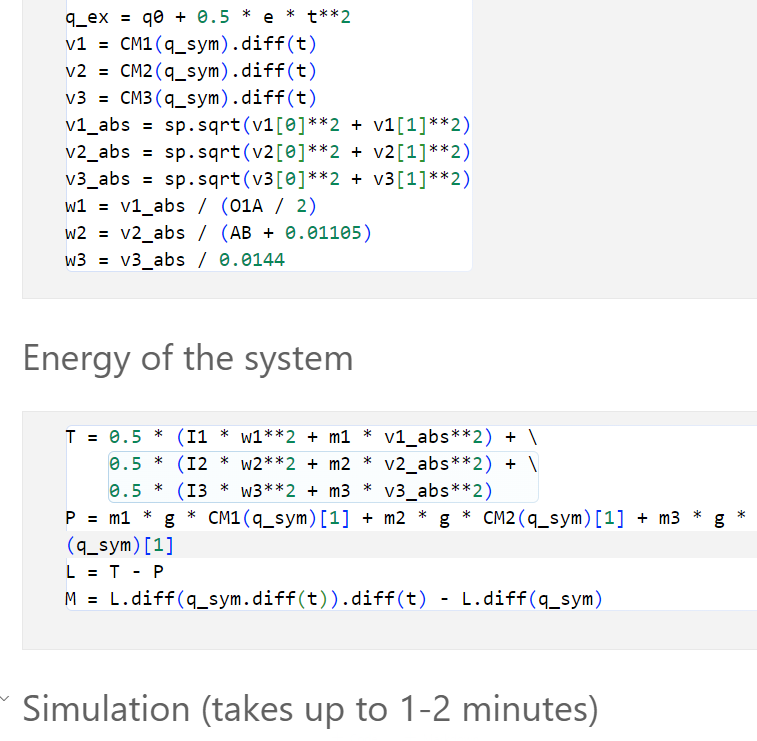
\includegraphics[height=6cm,width=1\textwidth,keepaspectratio]{code.png}
            \caption*{Coding}
            \label{fig:code.png}
        \end{subfigure}
        \begin{subfigure}[t]{0.32\textwidth}
            \centering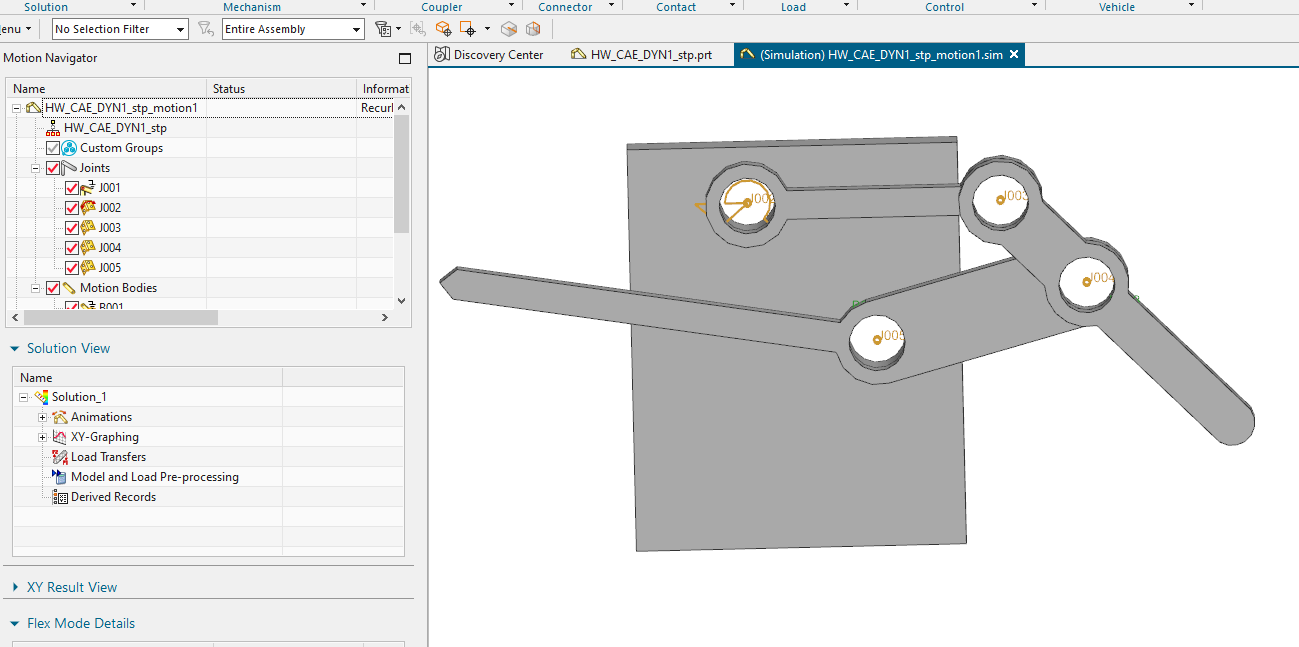
\includegraphics[height=6cm,width=1\textwidth,keepaspectratio]{nx.png}
            \caption*{Siemens NX (CAE)}
            \label{fig:nx.png}
        \end{subfigure}
        \begin{subfigure}[t]{0.32\textwidth}
            \centering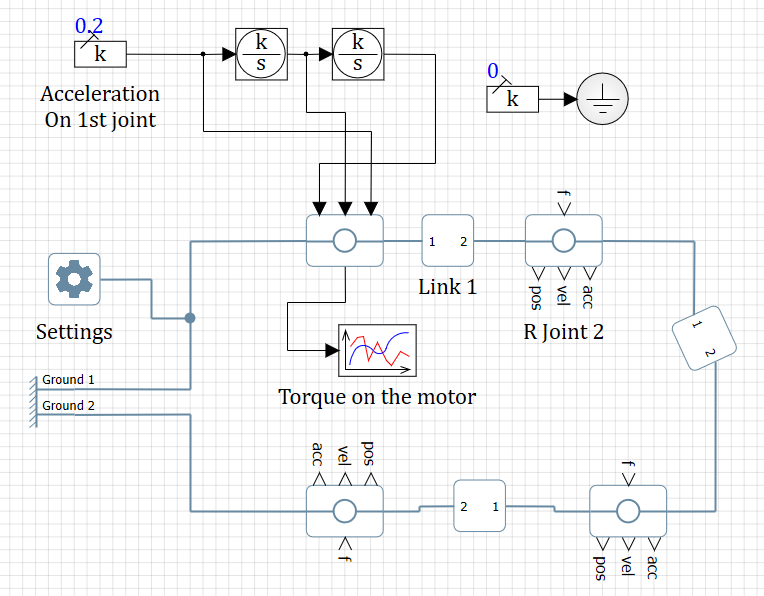
\includegraphics[height=6cm,width=1\textwidth,keepaspectratio]{simintech.png}
            \caption*{SimInTech (Model-oriented design)}
            \label{fig:simintech.png}
        \end{subfigure}
    \end{figure}
\end{frame}  

\begin{frame}[t]{Solution (2)}
\framesubtitle{}
    \vspace{-0.6cm}

    \begin{figure}[H]
        \begin{subfigure}{0.49\textwidth}
            \centering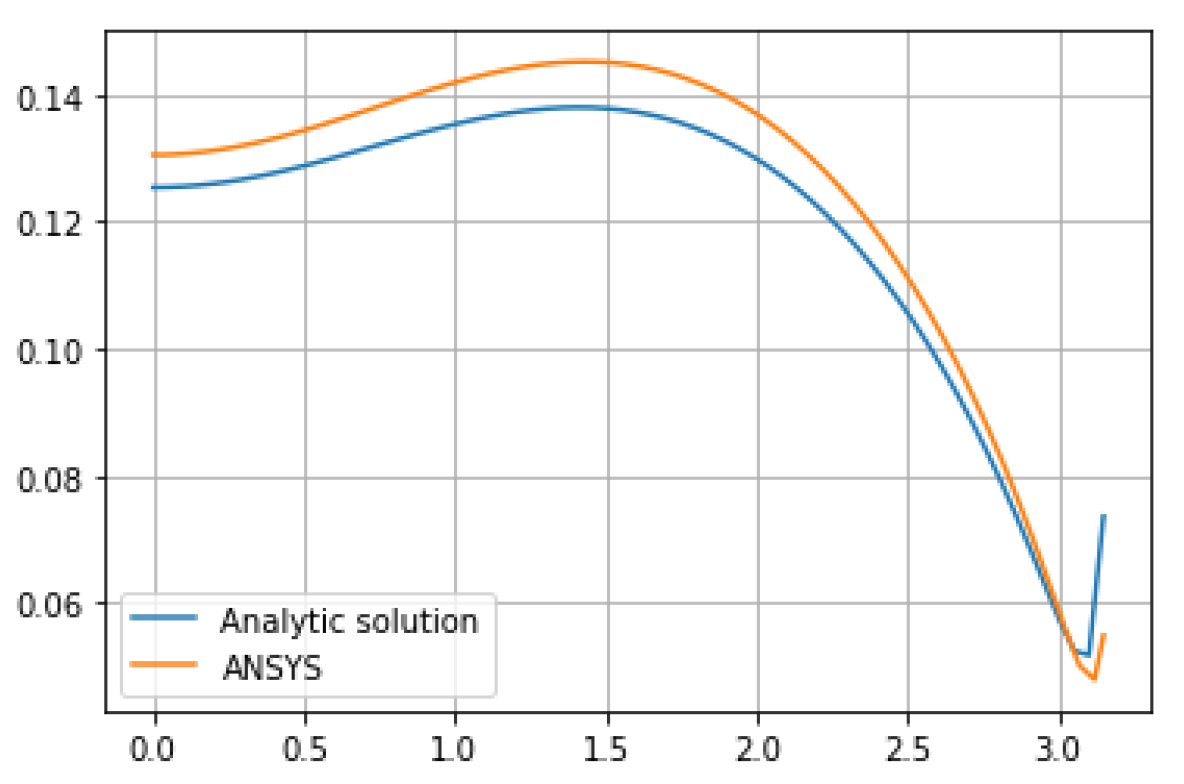
\includegraphics[height=6cm,width=1\textwidth,keepaspectratio]{plots_code_ansys.png}
            \caption*{Plots CAE and Code}
            \label{fig:plots_code_ansys.png}
        \end{subfigure}
        \begin{subfigure}{0.49\textwidth}
            \centering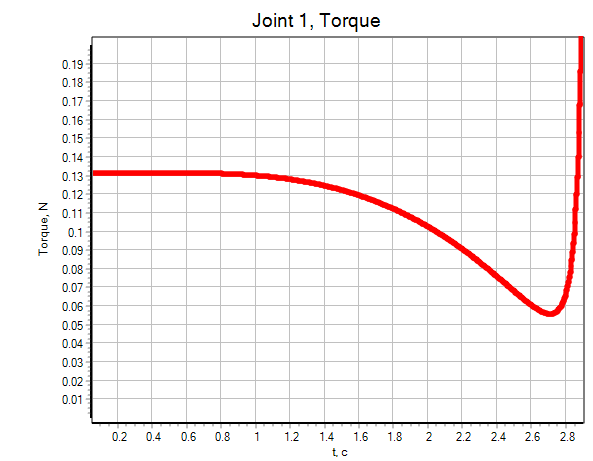
\includegraphics[height=6cm,width=1\textwidth,keepaspectratio]{plot_simintech.png}
            \caption*{Plot Model-oriented design}
            \label{fig:plot_simintech.png}
        \end{subfigure}
    \end{figure}
\end{frame}


\begin{frame}[t]{Two basic concepts of solving dynamics by coding (1)}
    \framesubtitle{}
        \vspace{-0.6cm}
        \begin{figure}[H]
            \centering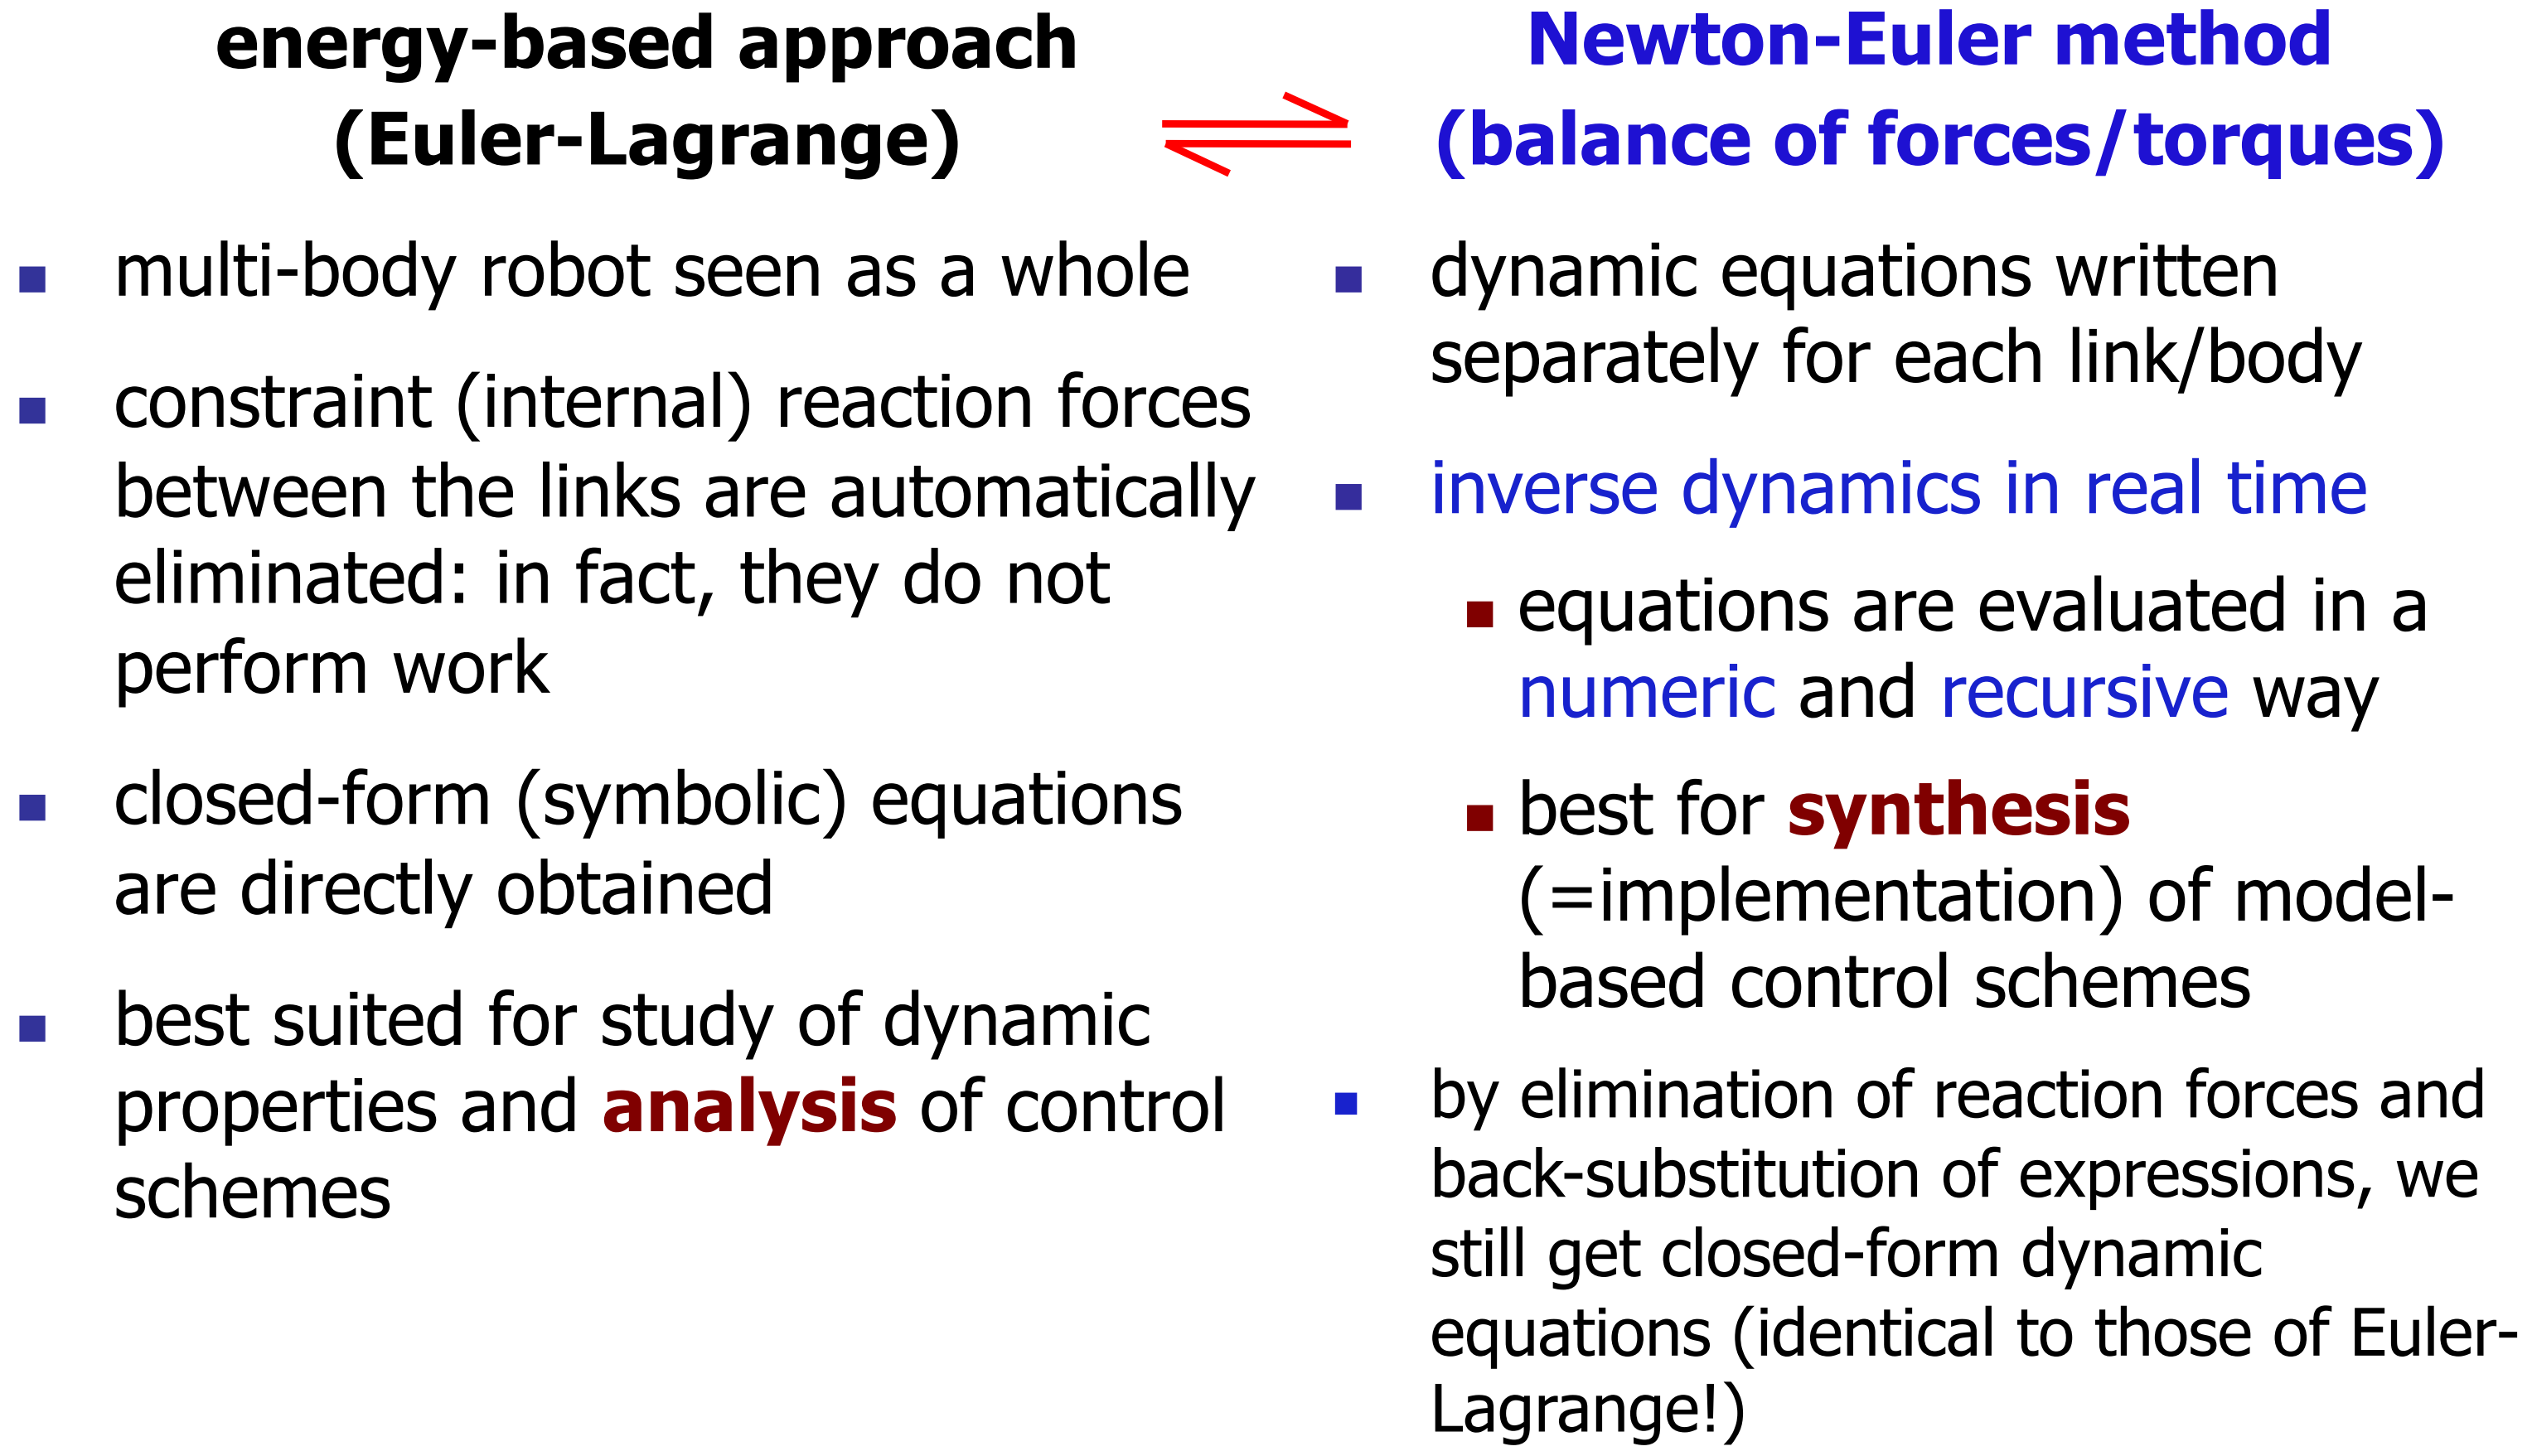
\includegraphics[height=6cm,width=1\textwidth,keepaspectratio]{two_approaches.png}
            \label{fig:two_approaches.png}
        \end{figure}
    \end{frame}
    
    \begin{frame}[t]{Two basic concepts of solving dynamics by coding (2)}
    \framesubtitle{}
        \vspace{-0.6cm}
        \begin{figure}[H]
            \centering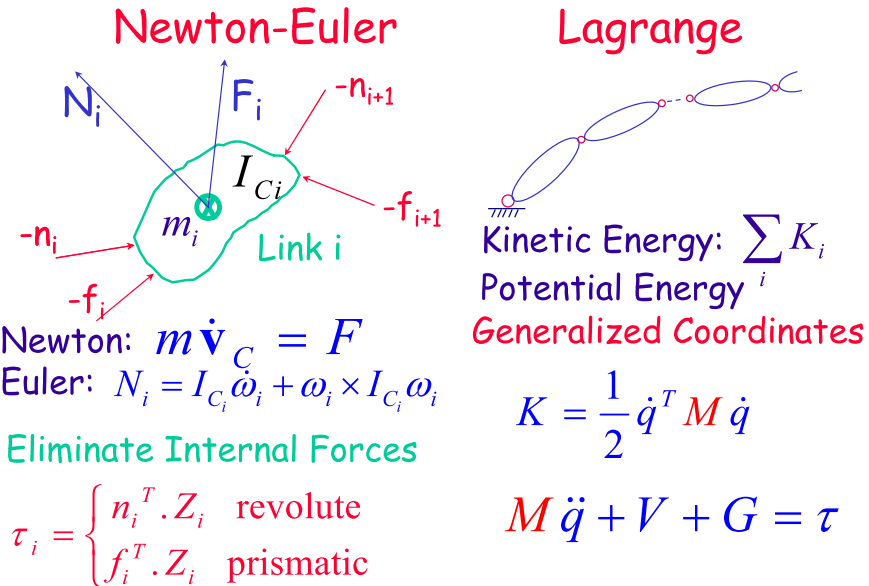
\includegraphics[height=6cm,width=1\textwidth,keepaspectratio]{image15.png}
            \label{fig:image15.png}
        \end{figure}
    \end{frame}
    
    \begin{frame}[t]{State of Art tools for coding}
    \framesubtitle{}
    Classical methods are rarely used in practice anymore, although new life has been breathed into them by the ability to use GPUs for computation.
    \medskip
    
    \textbf{Inverse dynamics} --- recursive Newton-Euler algorithm (RNEA).
    
    \textbf{Forward dynamics} --- articulated body algorithm (ABA), Kane's method, Composite Rigid Body Algorithm (for finding the M matrix) + RNEA.
    
    \textbf{For adding links} --- Featherstone algorithm or Lagrange multipliers.
    \medskip
    
    \textit{Libraries for automatic differentiation}: Jax, CasADi, PyTorch.
    
    \textit{Libraries for automated dynamics writing}: Pinocchio, Rigid Body Dynamics Library (RBDL).
    \end{frame}

\section*{Newton-Euler method}

\begin{frame}[t]{Newton-Euler method}
    \framesubtitle{}
    \scriptsize
        \begin{tabular}{>{\centering\arraybackslash} m{0.9cm}|>{\centering\arraybackslash} m{1.5cm}|>{\centering\arraybackslash} m{5.0cm}|>{\centering\arraybackslash} m{1.6cm}|>{\centering\arraybackslash} m{3cm} } 
            \toprule
            \toprule
           \textbf{ R. O.} & \textbf{Eqn \#} & \textbf{Equations} & \textbf{Applications} & \textbf{Extra Info} \\ 
            \hline
            \ExecuteMetaData[../../dynamics_methods_overview/dynamics_methods_overview]{sndnewtoneuler}
            \bottomrule
            \bottomrule
            \end{tabular}
    \end{frame}

\begin{frame}[t]{Task 1 (mine)}
\framesubtitle{}
    \begin{columns}[T,onlytextwidth]
        \begin{column}{0.49\textwidth}
            Determine the motion of the system. All needed parameters are given.
        \end{column}
        \begin{column}{0.49\textwidth}
            \vspace{-1cm}
            \begin{figure}[H]
                \centering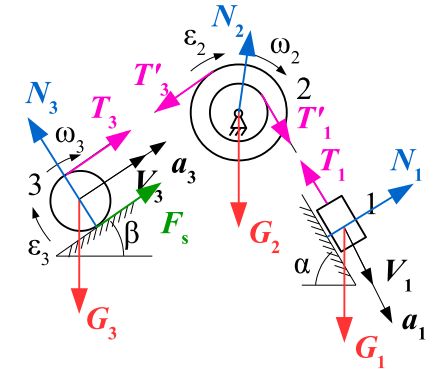
\includegraphics[height=6cm,width=1\textwidth,keepaspectratio]{im22.png}
                % \caption{caption_name}
                \label{fig:im22.png}
            \end{figure}
        \end{column}
    \end{columns}
\end{frame}

\begin{frame}[t]{Task 2 (yours): M (rus) 48.5 (answer only)}
\framesubtitle{}
\begin{columns}[T,onlytextwidth]
    \begin{column}{0.59\textwidth}
        Determine the motion of a mass $m$ hanging on a homogeneous cable of mass $m_1$ and length $l$. The cable is wound on a drum of radius $a$ and mass $m_2$.
        \medskip

        The axis of rotation is horizontal; friction is neglected, the mass of the drum is considered to be uniformly distributed along its rim. 
        
        At the initial moment $t=0$ the system was at rest, the length of the dangling part of the cable $l_0$.
        \bigskip

        \textit{Answer:} $(m+m_1+m_2)\ddot{x} = \dfrac{m_1}{l}gx + mg$
    \end{column}
    \begin{column}{0.39\textwidth}
        \begin{figure}[H]
            \centering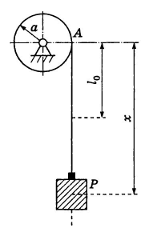
\includegraphics[height=5cm,width=1\textwidth,keepaspectratio]{im11.png}
            % \caption{caption_name}
            \label{fig:im11.png}
        \end{figure}
    \end{column}
\end{columns}    
\end{frame}


\begin{frame}[t]{Reference material}
\framesubtitle{}
    \begin{itemize}
        \item \href{https://www.diag.uniroma1.it/deluca/rob2_en.php}{Robotics 2 course, Sapienza Di Roma, Alessandro De Luca}
        \item \href{https://see.stanford.edu/Course/CS223A}{Introduction to Robotics, Stanford, Oussama Khatib}
        \item \href{https://simintech.ru/}{SimInTech}
        \item \href{https://help.simintech.ru/index.html?q=/15_demonstracionnye_primery/KEY_demonstracionnye_primery.html}{SimInTech examples of <<Mechanics>> and <<Mechanics 3D>> libraries}
        \item \href{https://www.mathworks.com/products/simulink.html}{MATLAB Simulink}
        \item \href{https://en.wikipedia.org/wiki/Siemens_NX}{Siemens NX}
    \end{itemize}
\end{frame}
\fbckg{fibeamer/figs/last_page.png}
\frame[plain]{}
\end{document}